Zwei Körper A und B starten zur Zeit $t = 0$ am selben Ort und bewegen sich auf einer geraden Linie. Das Diagramm zeigt ihre Geschwindigkeiten (A kehrt bei \tHO\ vereinfacht ohne Bremsweg um).
\begin{center}
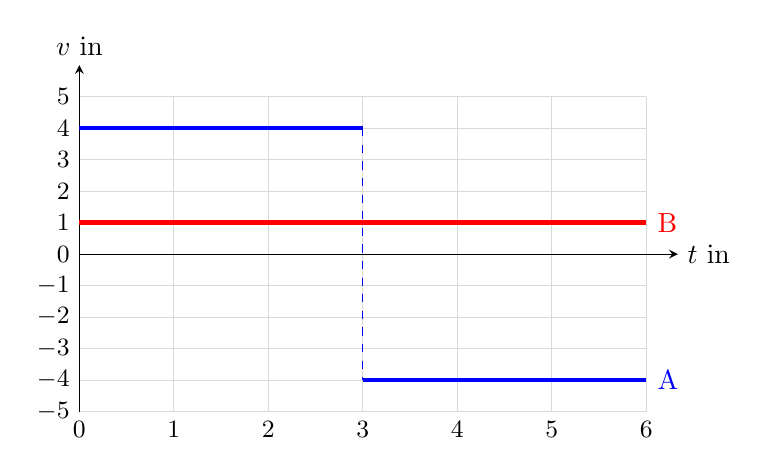
\begin{tikzpicture}[>=stealth, x=1.2cm, y=0.4cm]
 \draw[gray!30] (0,-5) grid[xstep=1, ystep=1] (6,5);
 \draw[->] (0,0) -- (6.333,0) node[right] {$t$ in \si{\second}};
 \draw[->] (0,-5) -- (0,6) node[above] {$v$ in \si{\meter\per\second}};
 \foreach \tk in {0,1,2,3,4,5,6} \node[below] at (\tk,-5) {\small $\tk$};
 \foreach \yk in {-5,-4,-3,-2,-1,0,1,2,3,4,5} \node[left] at (0,\yk) {\small $\yk$};

 \draw[ultra thick, blue] (0,4) -- (3,4);
 \draw[blue, dashed] (3,4) -- (3,-4);
 \draw[ultra thick, blue] (3,-4) -- (6,-4) node[right] {A};
 \draw[ultra thick, red] (0,1) -- (6,1) node[right] {B};
\end{tikzpicture}
\end{center}
\begin{abcliste}
\abc Wo befinden sich A und B zur Zeit \tEO, gemessen vom Startort?
\abc Welcher Körper ist bei \tEO\ weiter vom Startort entfernt?
\abc Noah meint: „A ist weiter weg, A ist ja \SI{24}{\meter} gefahren und B nur \SI{6}{\meter}.“ Was ist an seiner Überlegung falsch?
\end{abcliste}
